%Interaction between two individual elements in a system are %affected by the interface which is connecting the two parts.
There are different ways in which a system interact with it's environment and the other systems. The interaction happening at the various boundaries are called the system's external interfaces. The boundaries between individual components inside the system are called system's internal interfaces.\\
The external and internal identification can fall into different types such as: electrical, mechanical, real-time data transfer and storage-and-retrieval of data.

\subsubsection{External interfaces}
\begin{itemize}
\item {Interface identification and diagrams.}\\
\begin{figure}[h]
	\centering
	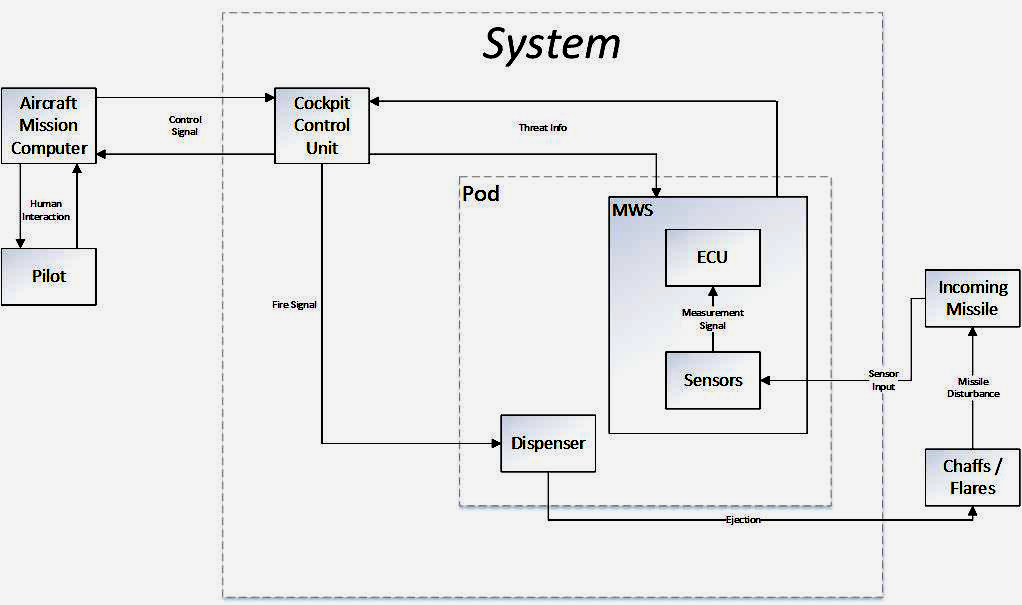
\includegraphics[scale=0.5]{./images/SignalFlowDiagram}\\
	\caption{Signal Flow Diagram}
    \label{fig:sigFlowDiagram}
\end{figure}

\item {Project-unique identifier of interface}\\
\begin{sidewaystable}[ht]
\begin{tabular}{ l l l l l l l }
\hline
%Environmental&&&&&&&&\\
&Type&Interaction medium&data element&communication methods&protocols&physical compatibility\\
\hline
Incoming missile&&&&&&\\
\hline
Chaffs and flares&&&&&&\\
\hline
Aircraft Mission Computers&&&&&&\\
\hline
System Operators&&&&&&\\
\hline
Maintenance&&&&&&\\
\hline
Support&&&&&&\\
\hline
System Housing&&&&&&\\
\hline
Shipping and handling&&&&&&\\
\hline
\end{tabular}
\caption{External Interface Elements}
\end{sidewaystable}[htbf]
%Electrical&Mechanical&Hydraulic
\end{itemize}


\subsubsection{Internal interfaces}
\begin{itemize}
\item{Interface identification and diagrams.}\\
blaa
\item{Project-unique identifier of interface}\\

\end{itemize}